
\subsubsection{The Micromegas ART Pattern Generator}

In order to properly test the full trigger electronics chain without
access to a large number of chambers, it is necessary to implement a
pattern generator  to simulate the ART (address in real time) output
from the VMM chips. This pattern generator will interface with the
ART Data Driver Card (ADDC), which will then transmit information via
fiber optic link to the Trigger Processor (TP).

The firmware for the ART Pattern Generator (APG) has been written and
is currently being tested on a Xilinx
Virtex 7 FPGA in a VC707 development board. Each development board has
FMC output connectors. A mezzanine
card has been developed to adapt these FMC connectors to the MiniSAS
connectors expected by the ADDC card.

The signal emulation will be accomplished by reformatting simulated
muon events in the NSW in Athena and sending them via an ethernet
interface to the FPGA. On the FPGA, the hits will be sorted to the
correct ART output and clocked out according to the timing indicated
in the event. Finally, the 6 bits of the strip number are output
serially through the FMC connector according to the LVDS standard
expected by the ADDC inputs. Figure~\ref{fig:artDataStimPG} shows the
general chain of the testing configuration using the APG and 
Figure~\ref{fig:APGBlockDiag} shows the full program flow of the APG from simulation to serialized output on the evaluation board FPGA.

\begin{figure}[h]
 \begin{center}
 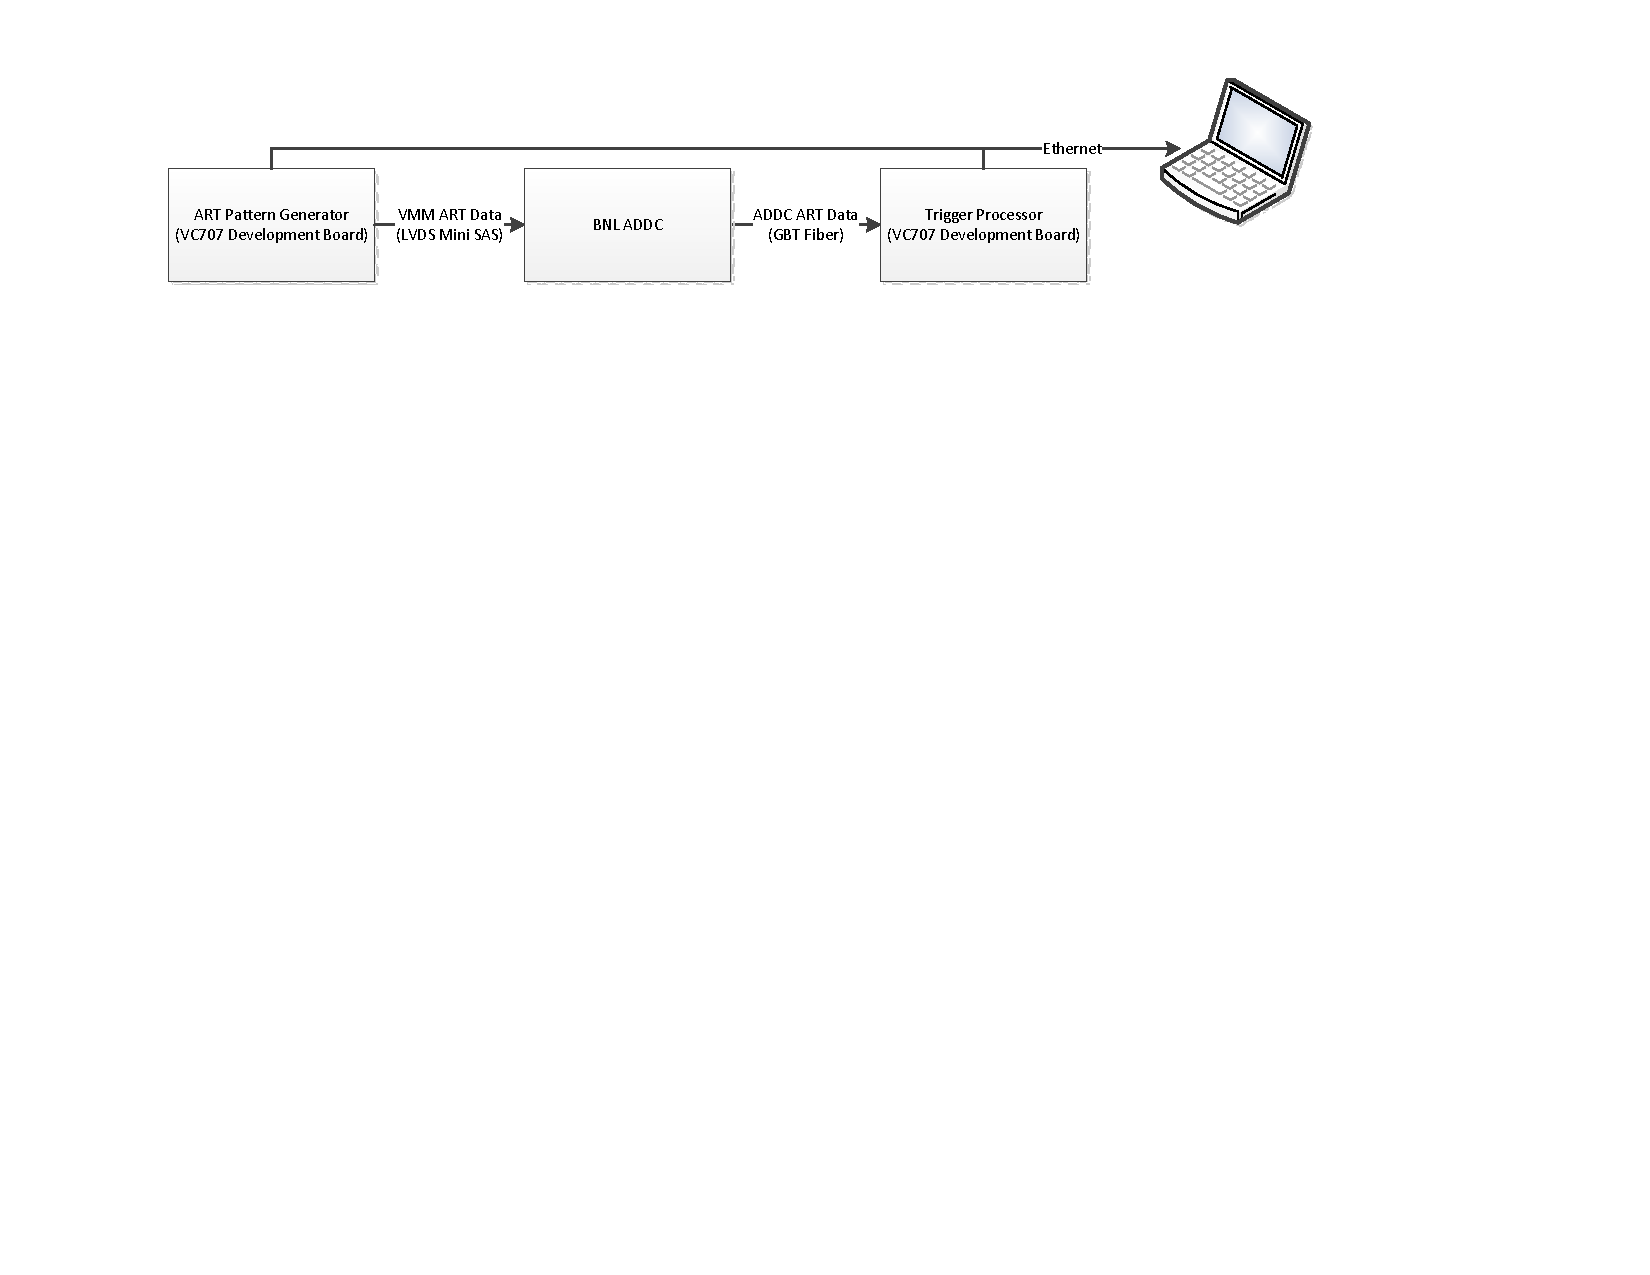
\includegraphics[width=0.9\textwidth]{figures/testing/artDataStimPG.pdf}
 \caption{Testing configuration for APG.}
 \label{fig:artDataStimPG}
 \end{center}
 \end{figure}

\begin{figure}[h]
 \begin{center}
 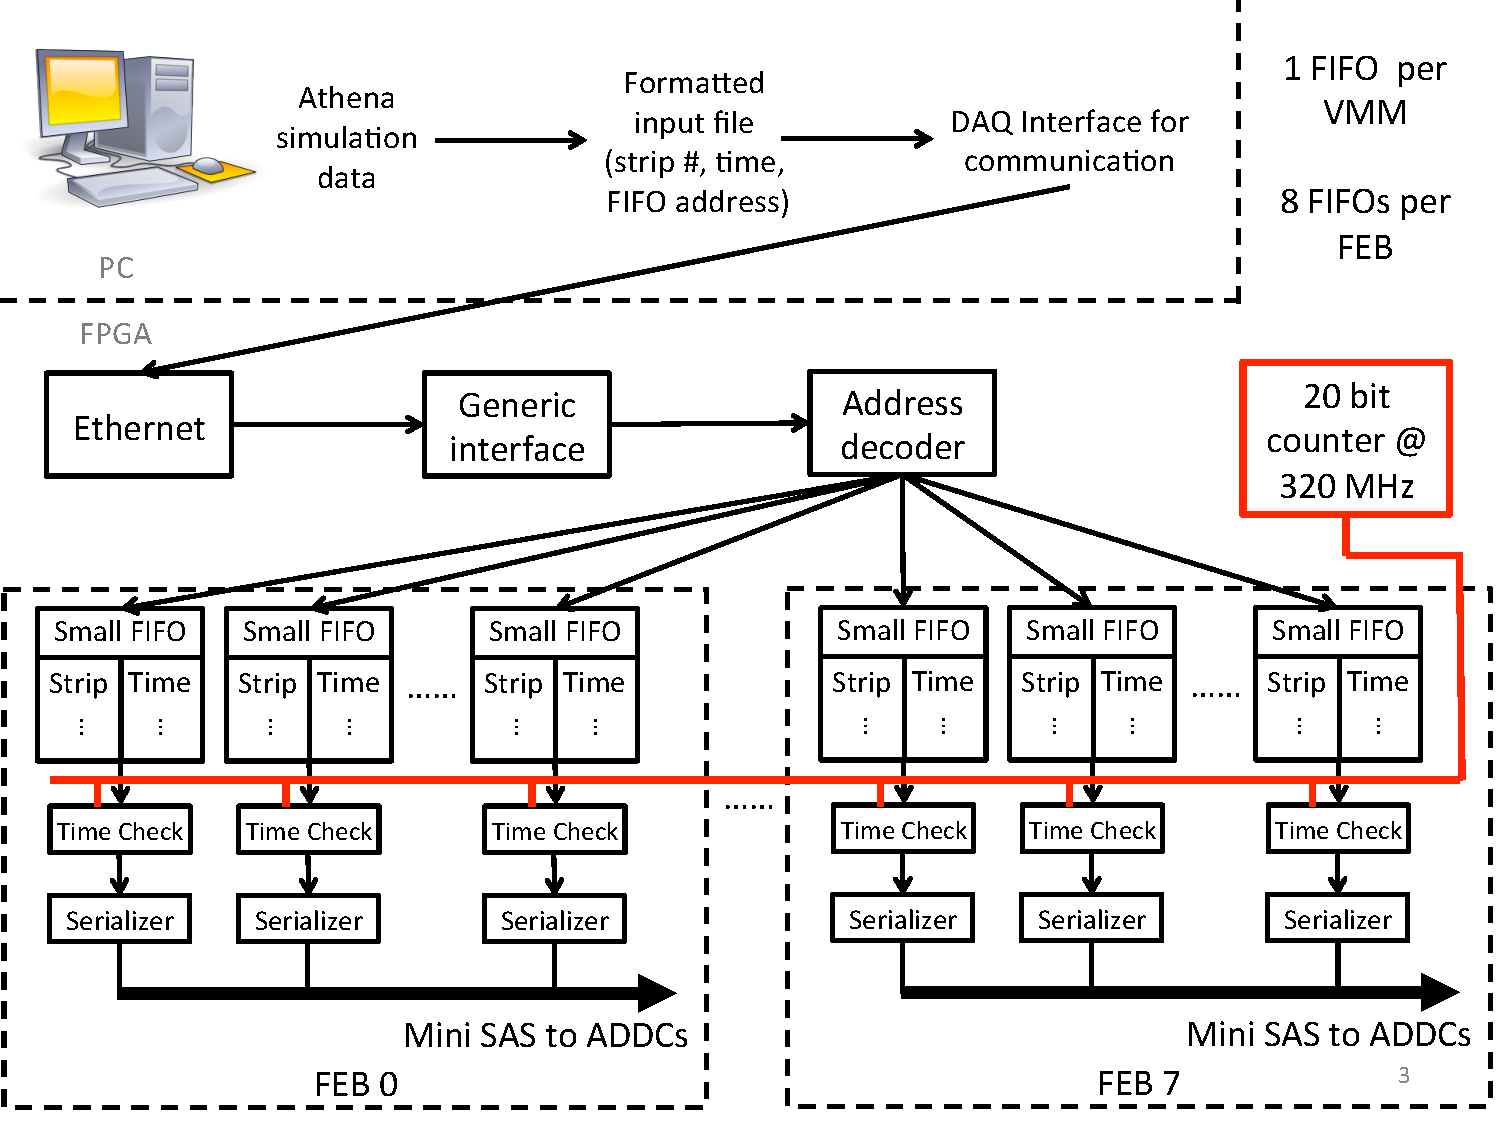
\includegraphics[width=0.9\textwidth]{figures/APGBlockDiagramFinal}
 \caption{Block diagram representing the detailed flow of the APG.}
 \label{fig:APGBlockDiag}
 \end{center}
 \end{figure}

The APG will be used in conjunction with the BNL ADDC and the trigger
processor to test the performance of the electronics and trigger
algorithm  as a function of various parameters of interest (including
track slope,  hit rates, etc.). Performance metrics for the algorithm
will include efficiency and fake rates. Performance metrics for the
electronics  will include latency measurements and stress tests with
large track and/or background rates.
\FloatBarrier

\subsubsection{The sTGC Pattern Generator}
\label{sec:sTGCpattern}

A Matlab program generates patterns for testing the sTGC algorithm.
Values for track angle, hit radius, hit intensity and hit $\phi$ position are taken from a uniform distribution within predefined limits.
The event parameters are then parsed into Trigger Processor algorithm inputs for each of the eight layers.
Figure\,\ref{fig:TGCevgen} shows a graphical representation of one quadruplet image of one generated event.
The expected algorithm output is calculated for each generated event for verification.

\begin{figure}[h]
   \centering
   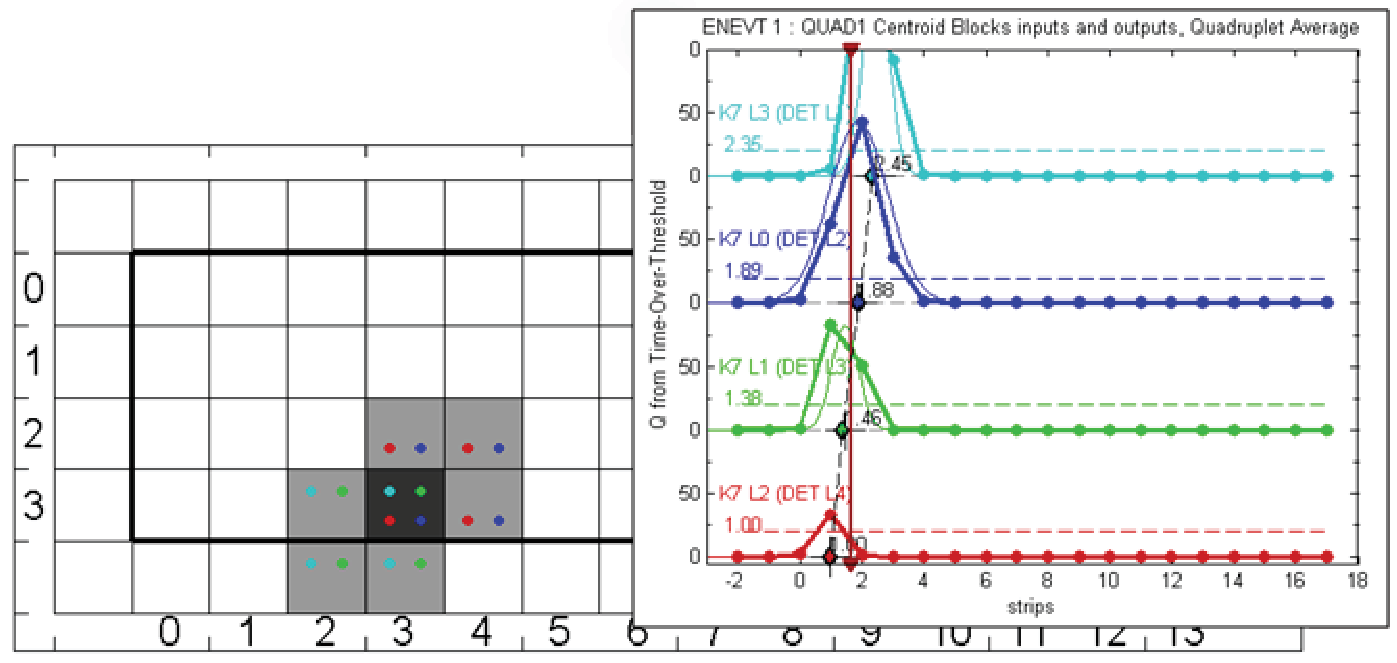
\includegraphics[width=0.8\textwidth]{figures/JN_TGCevgen_V01.pdf}
   \caption{An image on the background showing an active pad tower (defined by the overlapping pads shown in grey) as a dark square,
   where the dots indicate which of the layers in the pad tower have pad signals above threshold.
   The foreground image shows the pulse heights of the strips passing through the pad tower for this event.}
   \label{fig:TGCevgen}
\end{figure}

This mechanism was implemented on two identical sTGC trigger demo FPGA boards.
One board emulated the detector outputs using preloaded generated event data patterns for several events and the other was configured as the Trigger Processor.
In the next step towards algorithm testing,
simulated muon events from the ATLAS simulation program will be parsed into the sTGC Trigger Processor input pattern.
This will allow verification of the algorithm functionality and its optimization.
Using the same simulated events will also allow comparison between sTGC and \MM trigger processing algorithms.
As a final test, playback pattern generation will be employed in which real event data can be recorded and parsed as an input pattern.

\FloatBarrier


